\documentclass[a4paper,10pt]{article}
\usepackage[utf8]{inputenc}
\usepackage[margin=1.25in]{geometry}
\usepackage{setspace}
\newcommand{\grvis}{\texttt{GRVis}}
\doublespace
\title{\grvis : Visualization Framework for Computational General Relativity}
\author{Milinda Fernando (u1011531), Max Carlson (u0450449)}

\begin{document}

\maketitle

\section{Introduction}
%Give an overview of the project.
%Why is this project important and/or interesting
As gravitational waves from the merger of two black holes were detected in 2015, for the first time by the Advanced Laser Interferometry Gravitational-Wave Observatory (aLIGO) which spiked the interest in computational frameworks for computational general relativity, which enables to perform simulation on binary black hole merger problem. In this project, we would like to focus on developing an efficient, scalable visualization pipeline for our own research code Dendro(please note that current work is not published yet, but an extension of \cite{Fernando:2017:MAA:3078597.3078610}) which enables to solve BSSN\cite{2012PhRvD..85h4004B} formulation of Einstien equations in an efficient scalable manner, using octree based adaptive mesh refinement and with adaptive time stepping. 

BSSN formulation consists of $24$ non-linear hyperbolic PDE decomposition of Einstien equations which enables stable numerical time stepping. Hence each data files consists of $24$ evolution variables and $6$ constraint equations which are being used to test the physical validity of the solution. 

\begin{figure}[H]
	\centering
	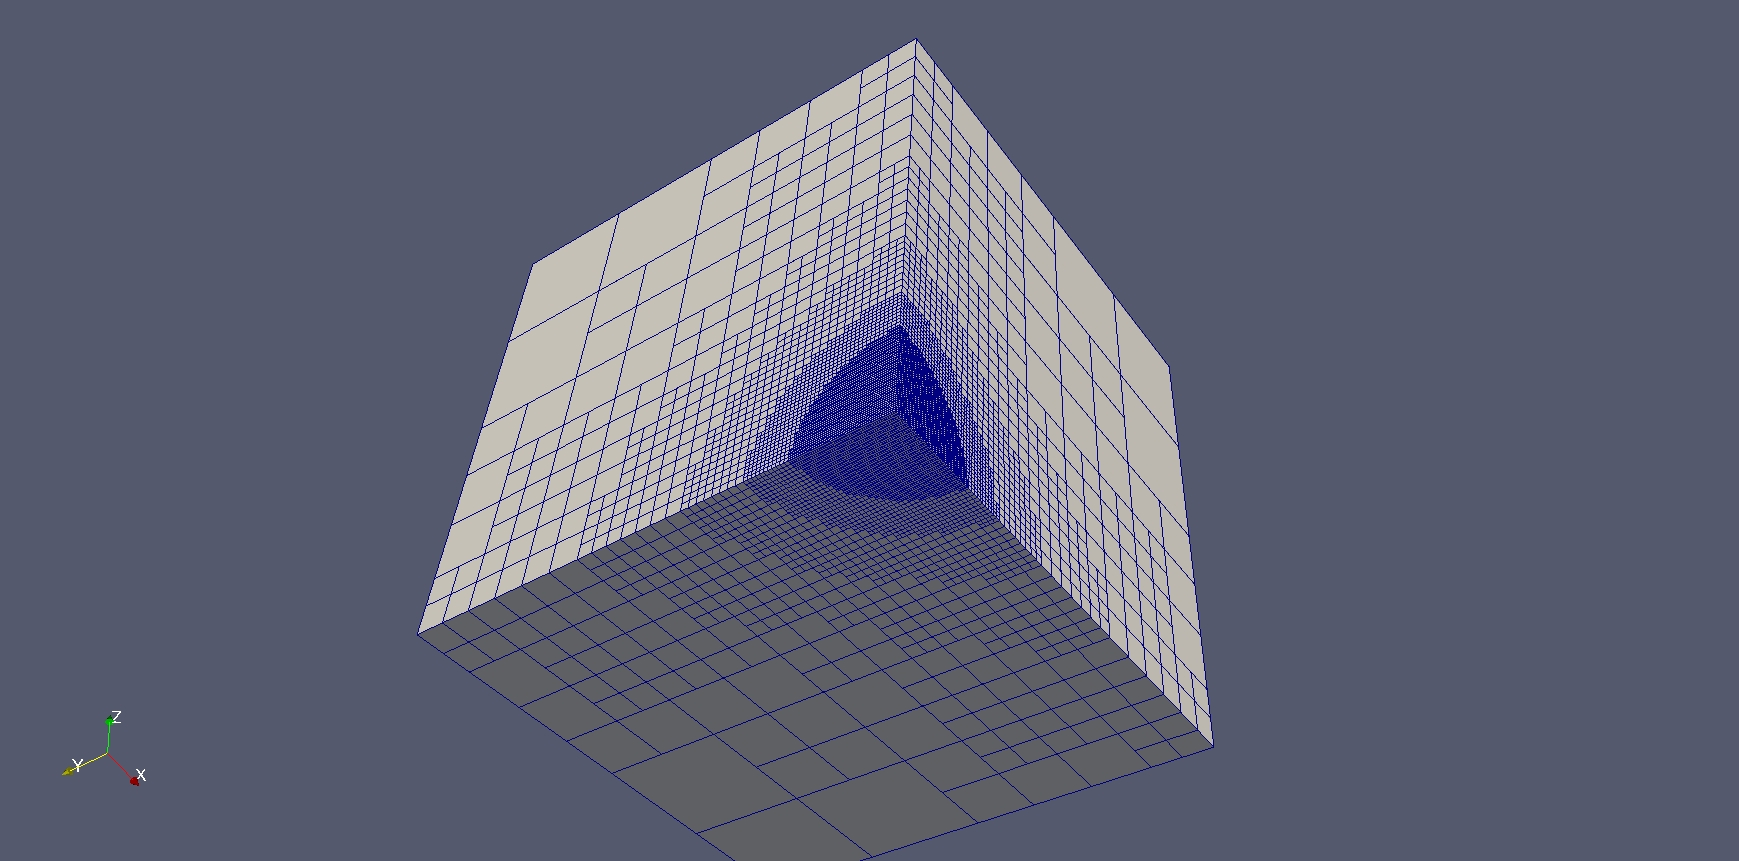
\includegraphics[width=0.45\textwidth]{figs/aoctree.jpg}  \hfill
	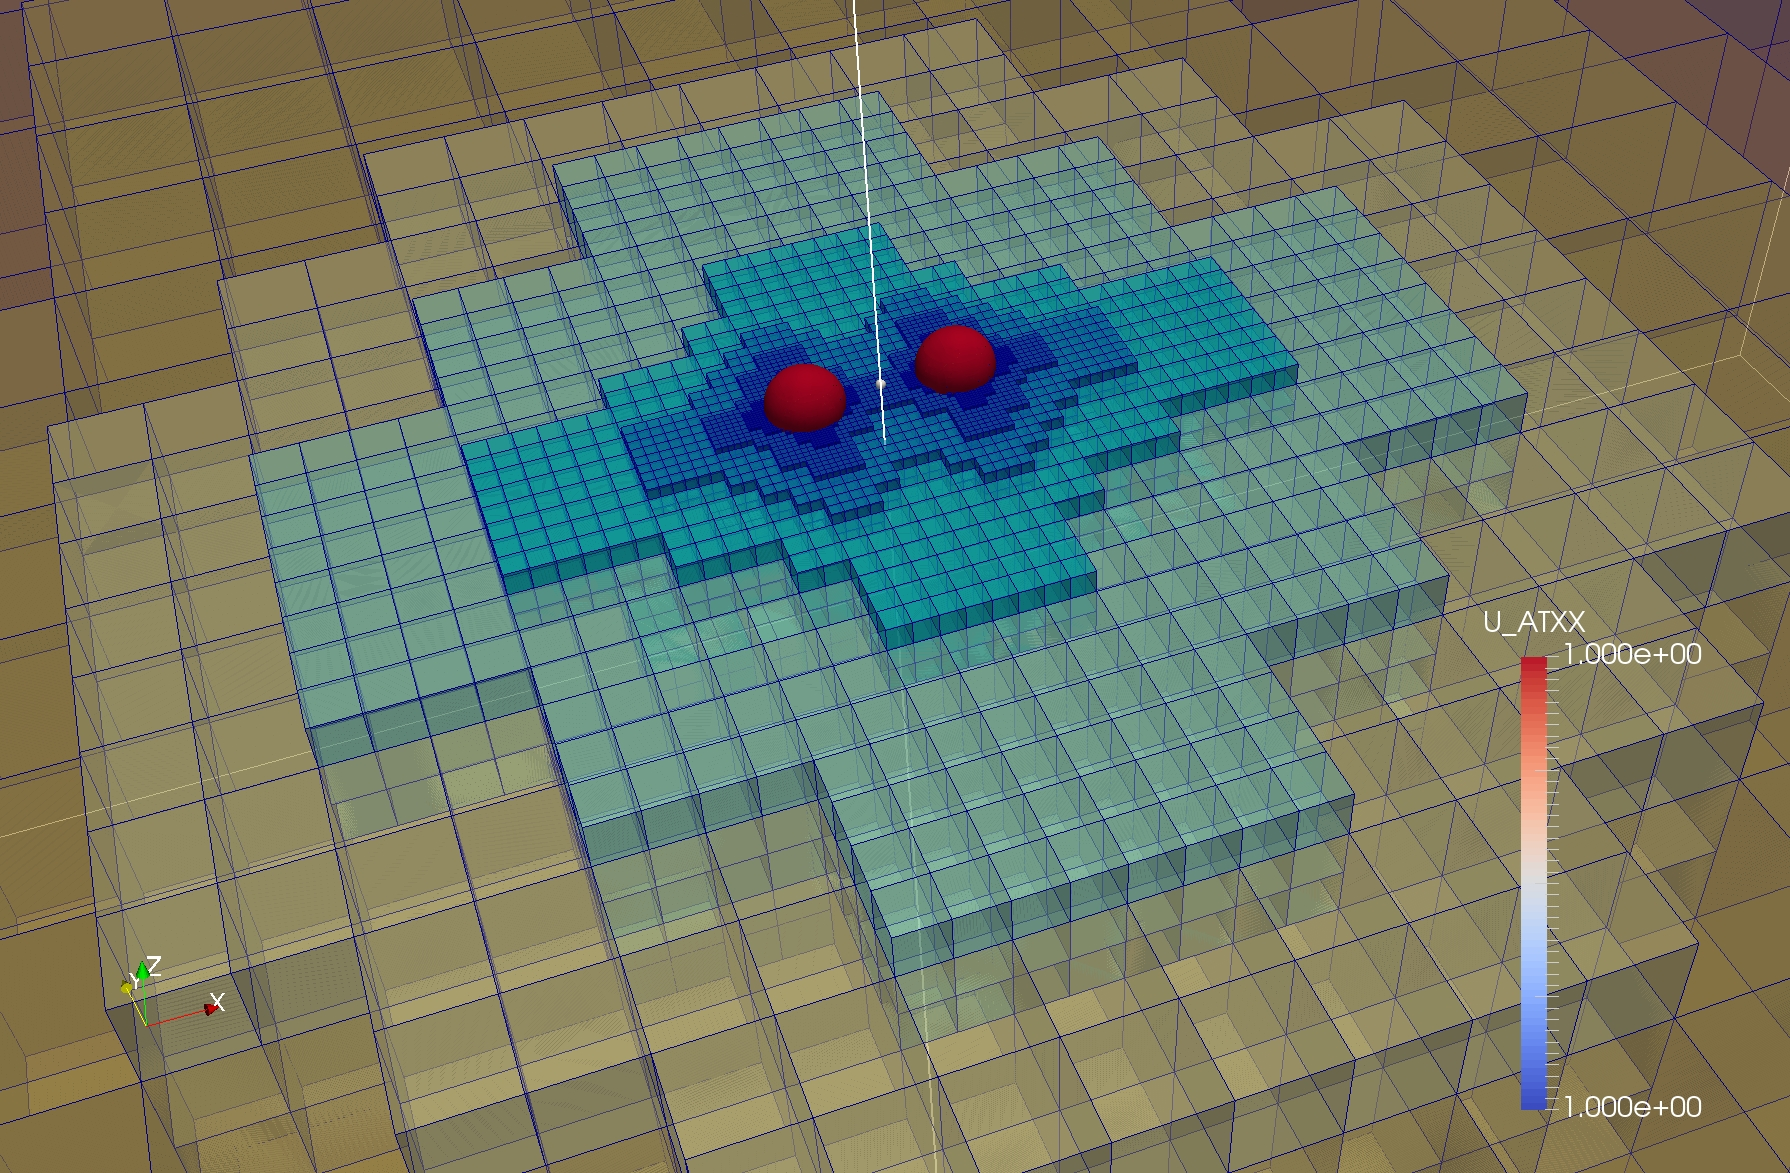
\includegraphics[width=0.45\textwidth]{figs/bh_image.jpg}
	\caption{\label{fig:octree} The leftmost figure shows an example of adaptive $2:1$ balanced octree and the rightmost image shows underlying adaptive grid for equal mass binary black hole problem.  }
\end{figure}

% What are the objectives of the project? What are the questions you want to answer?
% What would you like to learn by completing this projec
\section{Objectives}
The primary objective of this project is to develop a parallel rendering pipeline to quickly and easily generate animations from the data generated by the black hole simulation. Since the data has up to 24 output fields, analyzing the results is impractical without some form of visualization. This simulation is also of a very large size and can be run on thousands of nodes which can be a nightmare to debug. With a solid visualization pipeline, errors and unexpected behavior can be seen much more easily.

Since the work in this class is largely done using ParaView, and both of us have some experience rendering using parallel ParaView, this is also a good chance to compare ParaView and Visualization ToolKit (VTK) \cite{vtk}. For instance, knowing that ParaView is an extension of VTK, how much computational overhead does ParaView add? Does VTK make rendering in parallel easier or harder? These are two of the questions we intend to explore during the implementation of this project.

Finally, once we have a visualization pipeline in place, we can explore an advanced topic related to visualization such as In Situ Rendering, Fourth Order Tensor Visualization or other topics that may present themselves naturally during the course of implementation. This phase of the project will give us the opportunity to explore the data and perhaps find structures that are rarely visualized or potentially unknown.

%What data will you be using for your project
\section{Data}

%What is your project schedule? What have you done thus far and what will you have to do to
%complete this project? Be as specific as possible.
\section{Schedule}
For the given time frame, we will break up the project into two parts. The first part will consist of getting the python parallel rendering pipeline operational and will take place starting from March 15th until April 3rd when the first progress report is due. Then the second part, starting April 3rd until the due date April 19th, will involve extending this pipeline to cover an "advanced" topic which will be decided on when writing the progress report.

For part 1, the tentative schedule is

\begin{itemize}
	\item \textbf{March 15th through March 18th:} Get sequential VTK rendering examples running using single pvtu files from black hole simulation using python.
	\item \textbf{March 19th through March 23rd:} Extend the python script to render many pvtu files in parallel and stitch them together into a single image.
	\item \textbf{March 26th through March 30th:} Using the parallel python script, generate a few movies from the black hole data set. (single slice with warp by scalar, volume rendering, both combined)
	\item \textbf{April 2nd and April 3rd:} Write up project progress report and decide on focus for part 2.
\end{itemize}

Once part 1 is complete, we will choose an advanced topic to explore and implement. This topic will be chosen during the progress report write-up and will include an updated schedule for the final April 3rd to April 19th time frame Some of the potential advanced topics include

\begin{itemize}
	\item \textbf{In Situ Rendering:} Extend the GR code to use VTK to render the frames from memory to bypass file IO. Drastically reduces amount of data that needs to be stored and the data is already naturally partitioned among the same number of nodes and processes that generated it.
	\item \textbf{Rank-4 Tensor Visualization:} Using a tensor decomposition such as tucker decomposition, convert the Ricci rank-4 tensors into a form that can be visualized. If the tensors can be reduced to a collection of vector fields, a multi-field flow visualization would be very interesting to see.
\end{itemize}

%When the project is completed, how specifically can we evaluate how successful it is?
\section{Evaluation}

\bibliographystyle{unsrt}%Used BibTeX style is unsrt
\bibliography{grvis}

\end{document}
